%% -*- coding: utf-8 -*-
\documentclass[12pt,a4paper]{article} 
\usepackage[utf8]{inputenc}
\usepackage[english,russian]{babel}
\usepackage{indentfirst}
\usepackage{misccorr}
\usepackage{graphicx}
\usepackage{amsmath}
\begin{document}
\section{Введение}
\label{sec:intro}

% Что должно быть во введении
\begin{enumerate}
 \item Внесение в информационную базу 1С:Университет результатов сдачи зачётных и экзаминационных дисциплин студентов АГУ
 \item Порядок работы с системой.
 \item Скриншоты этапов работы с программой.
\end{enumerate}

\newpage
\section{Ход работы}
\label{sec:exp}

\subsection{Порядок работы в 1С:Университет}
\label{sec:exp:code}
Для заполнения ведомости необходимо: (скриншот 1)
\begin{enumerate}
			\item Перейти во вкладку "Управление студенческим составом".
            \item Произвести выборку по следующим параметрам: "Факульет", "Форма обучения", "Курс", "Группа", "Подгруппа" (при необходимости).
            \item В открывшемся окне выбрать необходимую аттестационную ведомость по следующим параметрам: "Предмет", "Форма оценивания".
\end{enumerate}

\subsection{Процесс заполнения аттестационной ведомости}
\label{sec:mathexample}

В выбранной аттестационной ведомости необходимо произвести следующие действия: (скриншот 2-3)
\begin{enumerate}
 			\item В соответствующем окне указать дату и время проведения экзамена / зачёта.
            \item В соответствующем окне указать преподавателя, принимавшего экзамен / зачёт.
            \item В соответствующем окне указать / сверить формат сдачи предмета (экзамен / зачёт).
            \item В соответствующем окне указать / сверить систему оценивания сдачи предмета (двубальную, пятибальную).
			\item В выделенном списке заполнить / сверить с имеющимся список студентов.
            \item Перенести  результаты в соответствии с бумажным носителем.
  			\item Осуществить контрульную проввеку внесенных / выбранных данных.
            \item Провести, сохранить и закрыть текущую ведомость.
\end{enumerate}

\newpage
\section{Скриншоты работ}
\label{sec:picexample}
\begin{figure}[h]
 \centering
 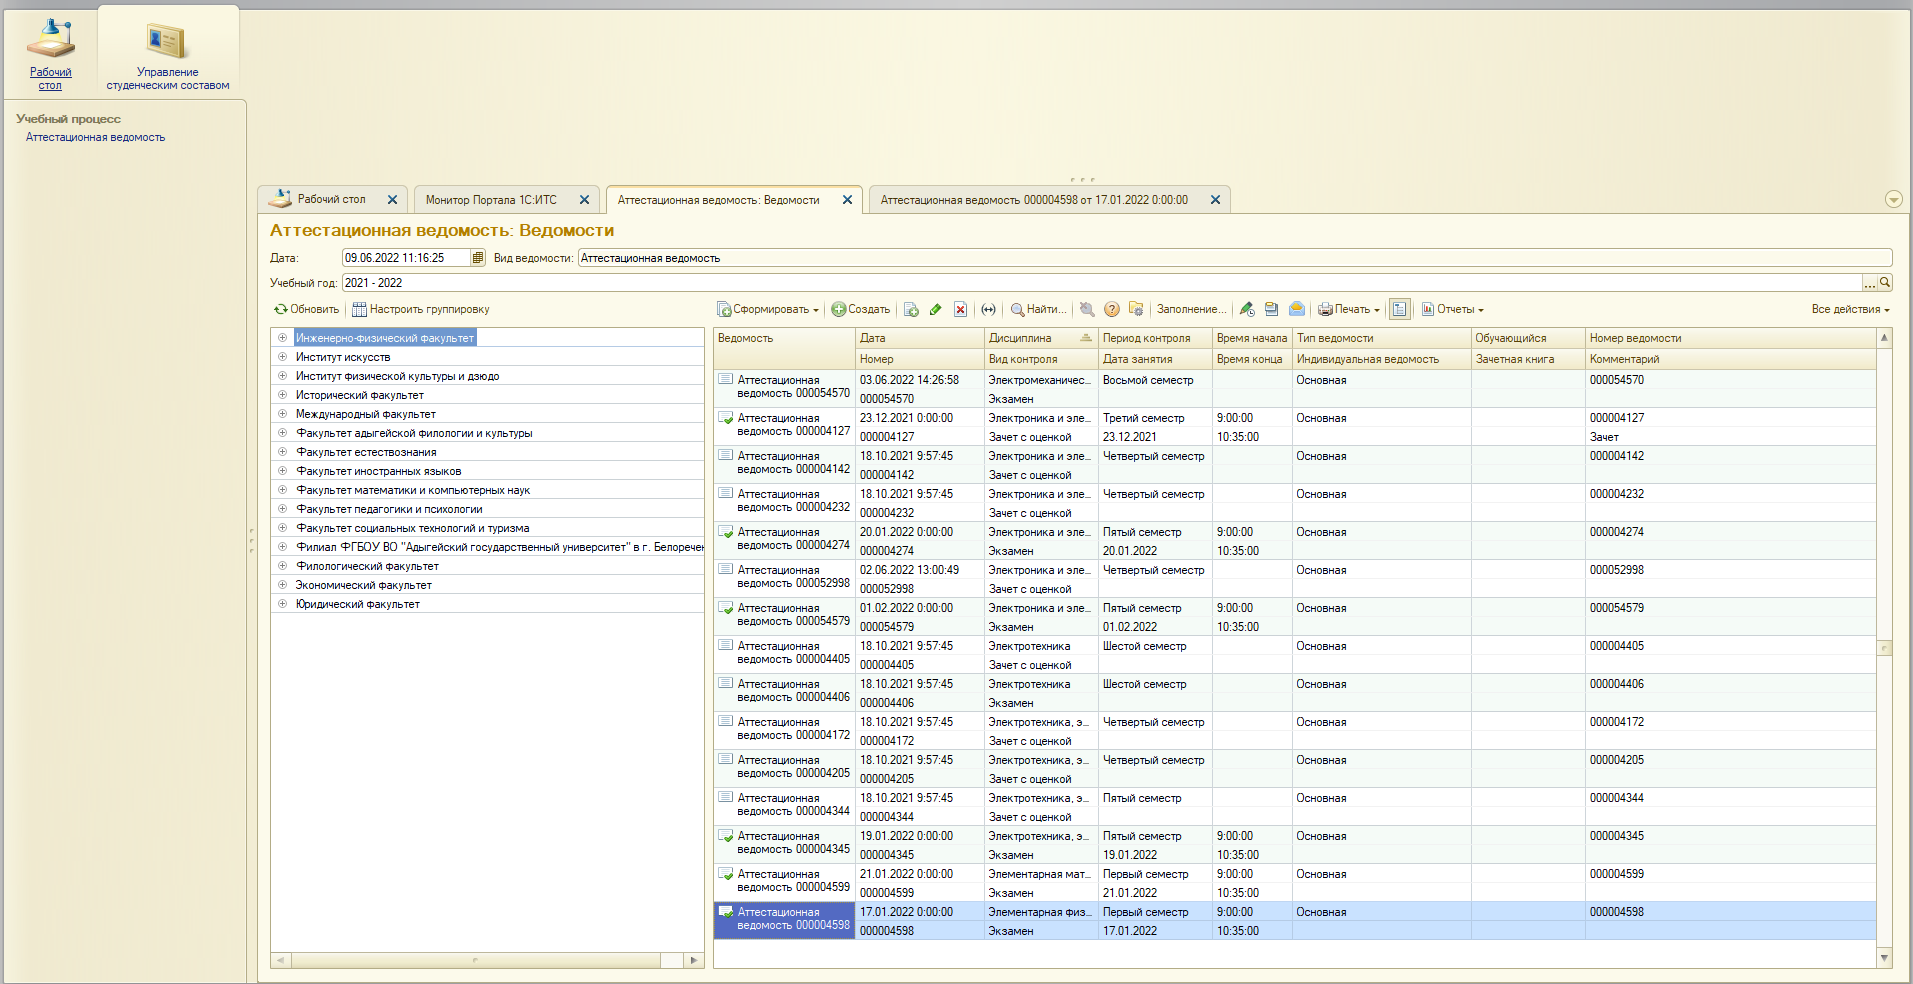
\includegraphics[width=0.9 \textwidth]{Pic3.png}
 \caption{Список аттестационных ведомостей (Скриншот 1)}\label{fig:par}
\end{figure}

\begin{figure}[h]
 \centering
 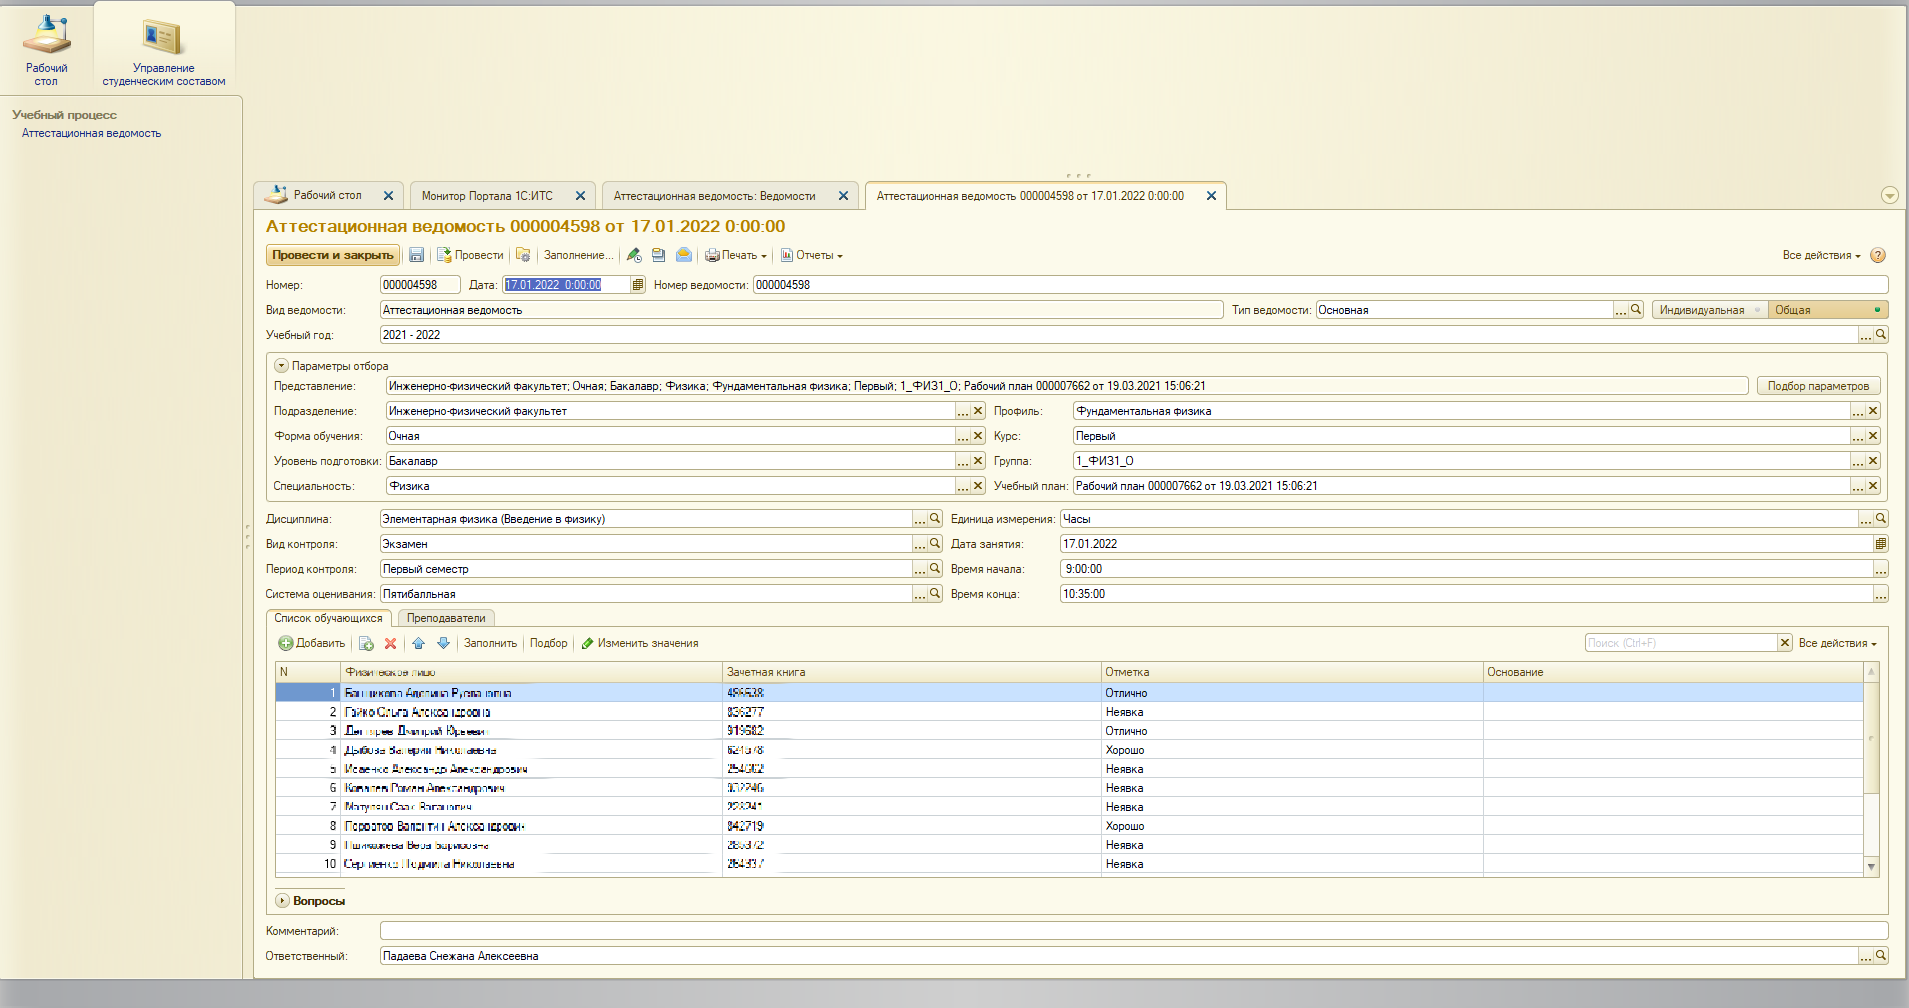
\includegraphics[width=0.9 \textwidth]{Pic2.png}
 \caption{Внутренние данные ведомости (Скриншот 2)}\label{fig:par}
\end{figure}

\begin{figure}[h]
 \centering
 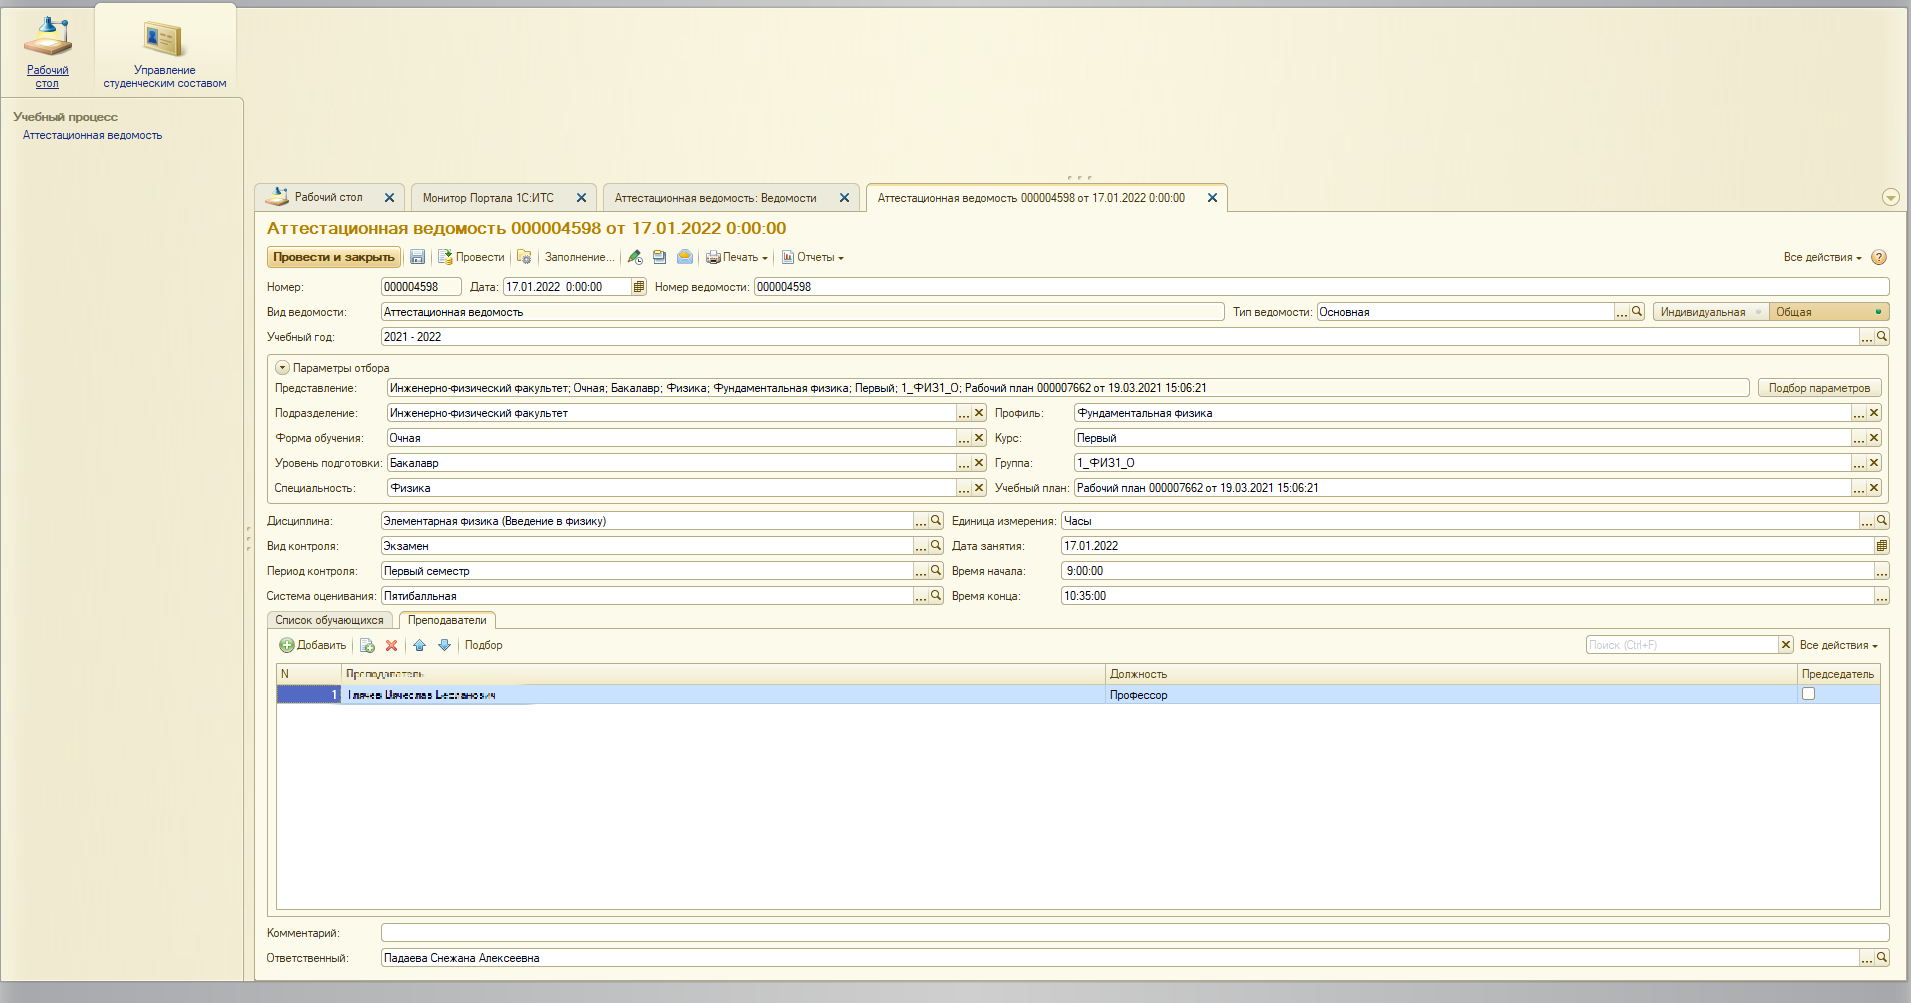
\includegraphics[width=0.9 \textwidth]{Pic1.png}
 \caption{Внутренние данные ведомости (Скриншот 3)}\label{fig:par}
\end{figure}

\end{document}
